\documentclass[10pt]{beamer}

\usepackage[utf8]{inputenc}
\usepackage[T1]{fontenc}
\usepackage{amsmath}
\usepackage{amsthm}
\usepackage{dsfont}
\usepackage{graphicx}
\usepackage{interval}
\usepackage{color}
\usepackage{xcolor,colortbl}
\usepackage[style=authoryear, maxcitenames=11, mincitenames=11, natbib=true, uniquename=false, uniquelist=false]{biblatex}
\addbibresource{main.bib}
\usepackage{multirow}
\usepackage{booktabs}
\usepackage{tikz}
\usetikzlibrary{patterns}
\usetikzlibrary{positioning}
\usetikzlibrary{decorations.pathreplacing,angles,quotes}
\usepgflibrary{arrows.meta,shapes.geometric}
\usepackage{algorithm}
\usepackage{algorithmicx}
\usepackage[noend]{algpseudocode}
\usepackage{dirtytalk}
\usepackage{hyperref}

\beamertemplatenavigationsymbolsempty%
\addtobeamertemplate{navigation symbols}{}{%
    \usebeamerfont{footline}%
    \usebeamercolor[fg]{footline}%
    \hspace{1em}%
    \insertframenumber/\inserttotalframenumber%
}

\author{Florian Fontan}
\title{Advanced Models and Methods in Operations Research \\ Heuristic Tree Search}
\date{November 16, 2021}

\begin{document}

\newcommand{\customcite}[1]{\citetitle{#1}, \citeauthor{#1}, \citeyear{#1}}

\AtBeginSection[]
{%
  \begin{frame}<beamer>
    \frametitle{Table of contents}
    \tableofcontents[currentsection]
  \end{frame}
}

\maketitle

\section{Introduction}

\begin{frame}
  \frametitle{Overview}

  Heuristic tree search is an optimization method based on the exploration of a search tree. It is made of two ingredients: \pause
  \begin{itemize}
    \item Branching scheme: representing the search space as an implicit decision tree. \pause
    \item Tree Search algorithm: exploring this search tree in a smart way to visit the most promising regions in priority
  \end{itemize}
\end{frame}

\section{Branching schemes}

\begin{frame}
  \frametitle{Definition}

  Branching scheme: representing the search space as an implicit decision tree.

  \bigskip

  A branching scheme is defined by:
  \begin{itemize}
    \item Its root node
    \item How to generate the children of a node
  \end{itemize}
\end{frame}

\begin{frame}
  \frametitle{Example: Travelling Salesman Problem}

  \small
  \begin{itemize}
    \item Input:
      \begin{itemize}
        \item $n$ locations
        \item an $n \times n$ symmetric matrix containing the distances between each pair of locations
      \end{itemize}
    \item Problem: find a tour such that each location is visited exactly once
    \item Objective: minimize the total length of the tour
  \end{itemize}

  \centering
  \begin{minipage}[t]{0.30\linewidth}
    \pause
    \centering
    Instance
    \bigskip

    \def\svgwidth{\columnwidth}
    \input{travelling_salesman_instance.pdf_tex}
  \end{minipage}
  \hspace{1cm}
  \begin{minipage}[t]{0.30\linewidth}
    \pause
    \centering
    Solution
    \bigskip

    \def\svgwidth{\columnwidth}
    \input{travelling_salesman_solution.pdf_tex}
  \end{minipage}
\end{frame}

\begin{frame}
  \frametitle{Example: Travelling Salesman Problem}

  Branching scheme
  \begin{itemize}
    \item A node corresponds to a partial tour
    \item Root node: contains only location $1$
    \item Children of a node: append to the partial tour the next location to visit; generate one child for each remaining location to visit
  \end{itemize}

  \pause
  Example with 4 nodes:
  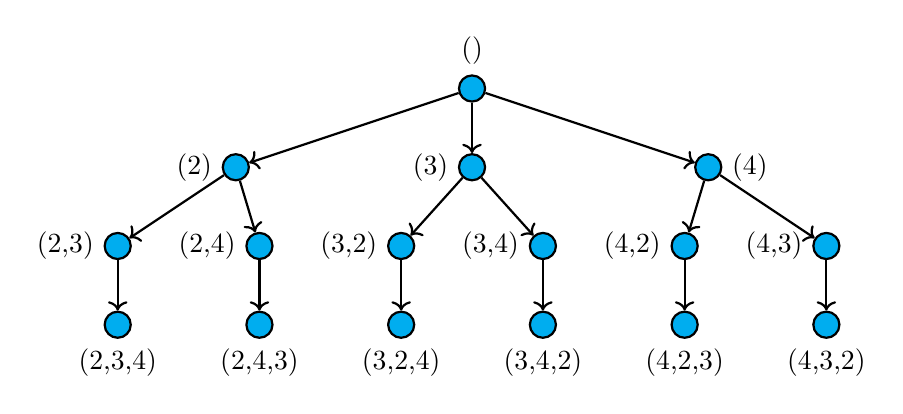
\begin{tikzpicture}
    \node[draw=black, thick, circle, fill=cyan, label=above:{()}] (N1) at (0,0) {};
    \node[draw=black, thick, circle, fill=cyan, label=left:{(2)}] (N12) at (-3,-1) {};
    \node[draw=black, thick, circle, fill=cyan, label=left:{(3)}] (N13) at (0,-1) {};
    \node[draw=black, thick, circle, fill=cyan, label=right:{(4)}] (N14) at (3,-1) {};
    \draw [thick, draw=black, ->] (N1) -- (N12);
    \draw [thick, draw=black, ->] (N1) -- (N13);
    \draw [thick, draw=black, ->] (N1) -- (N14);
    \node[draw=black, thick, circle, fill=cyan, label=left:{(2,3)}] (N123) at (-4.5,-2) {};
    \node[draw=black, thick, circle, fill=cyan, label=left:{(2,4)}] (N124) at (-2.7,-2) {};
    \node[draw=black, thick, circle, fill=cyan, label=left:{(3,2)}] (N132) at (-0.9,-2) {};
    \node[draw=black, thick, circle, fill=cyan, label=left:{(3,4)}] (N134) at (0.9,-2) {};
    \node[draw=black, thick, circle, fill=cyan, label=left:{(4,2)}] (N142) at (2.7,-2) {};
    \node[draw=black, thick, circle, fill=cyan, label=left:{(4,3)}] (N143) at (4.5,-2) {};
    \draw [thick, draw=black, ->] (N12) -- (N123);
    \draw [thick, draw=black, ->] (N12) -- (N124);
    \draw [thick, draw=black, ->] (N13) -- (N132);
    \draw [thick, draw=black, ->] (N13) -- (N134);
    \draw [thick, draw=black, ->] (N14) -- (N142);
    \draw [thick, draw=black, ->] (N14) -- (N143);
    \node[draw=black, thick, circle, fill=cyan, label=below:{(2,3,4)}] (N1234) at (-4.5,-3) {};
    \node[draw=black, thick, circle, fill=cyan, label=below:{(2,4,3)}] (N1243) at (-2.7,-3) {};
    \node[draw=black, thick, circle, fill=cyan, label=below:{(3,2,4)}] (N1324) at (-0.9,-3) {};
    \node[draw=black, thick, circle, fill=cyan, label=below:{(3,4,2)}] (N1342) at (0.9,-3) {};
    \node[draw=black, thick, circle, fill=cyan, label=below:{(4,2,3)}] (N1423) at (2.7,-3) {};
    \node[draw=black, thick, circle, fill=cyan, label=below:{(4,3,2)}] (N1432) at (4.5,-3) {};
    \draw [thick, draw=black, ->] (N123) -- (N1234);
    \draw [thick, draw=black, ->] (N124) -- (N1243);
    \draw [thick, draw=black, ->] (N132) -- (N1324);
    \draw [thick, draw=black, ->] (N134) -- (N1342);
    \draw [thick, draw=black, ->] (N142) -- (N1423);
    \draw [thick, draw=black, ->] (N143) -- (N1432);
  \end{tikzpicture}
\end{frame}

\begin{frame}
  \frametitle{Example: Sequential Ordering Problem}

  \begin{itemize}
    \item Input:
      \begin{itemize}
        \item $n$ locations
        \item an $n \times n$ matrix containing the distances between each pair of locations (not necessarily symmetric)
        \item a directed acyclic graph $G$ such that each vertex corresponds to a location
      \end{itemize}
    \item Problem: find a route from location 1 such that:
      \begin{itemize}
        \item each location is visited exactly once
        \item if there exists an arc from vertex $j_1$ to vertex $j_2$ in G, then location $j_1$ is visited before location $j_2$
      \end{itemize}
    \item Objective: minimize the total length of the route
  \end{itemize}
\end{frame}

\begin{frame}
  \frametitle{Example: Sequential Ordering Problem}

  \begin{itemize}
    \item Same branching scheme as for the Travelling Salesman Problem.
  \end{itemize}

  \pause

  Example with 5 nodes, precedences: $2 \to 5$, $3 \to 4$:
  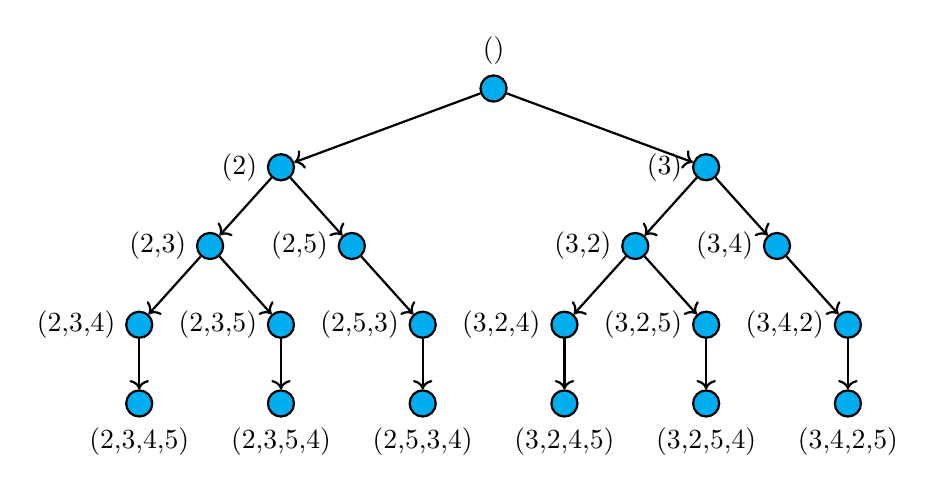
\begin{tikzpicture}
    \node[draw=black, thick, circle, fill=cyan, label=above:{()}] (N1) at (0,0) {};
    \node[draw=black, thick, circle, fill=cyan, label=left:{(2)}] (N12) at (-2.7,-1) {};
    \node[draw=black, thick, circle, fill=cyan, label=left:{(3)}] (N13) at (2.7,-1) {};
    \draw [thick, draw=black, ->] (N1) -- (N12);
    \draw [thick, draw=black, ->] (N1) -- (N13);
    \node[draw=black, thick, circle, fill=cyan, label=left:{(2,3)}] (N123) at (-3.6,-2) {};
    \node[draw=black, thick, circle, fill=cyan, label=left:{(2,5)}] (N125) at (-1.8,-2) {};
    \node[draw=black, thick, circle, fill=cyan, label=left:{(3,2)}] (N132) at (1.8,-2) {};
    \node[draw=black, thick, circle, fill=cyan, label=left:{(3,4)}] (N134) at (3.6,-2) {};
    \draw [thick, draw=black, ->] (N12) -- (N123);
    \draw [thick, draw=black, ->] (N12) -- (N125);
    \draw [thick, draw=black, ->] (N13) -- (N132);
    \draw [thick, draw=black, ->] (N13) -- (N134);
    \node[draw=black, thick, circle, fill=cyan, label=left:{(2,3,4)}] (N1234) at (-4.5,-3) {};
    \node[draw=black, thick, circle, fill=cyan, label=left:{(2,3,5)}] (N1235) at (-2.7,-3) {};
    \node[draw=black, thick, circle, fill=cyan, label=left:{(2,5,3)}] (N1253) at (-0.9,-3) {};
    \node[draw=black, thick, circle, fill=cyan, label=left:{(3,2,4)}] (N1324) at (0.9,-3) {};
    \node[draw=black, thick, circle, fill=cyan, label=left:{(3,2,5)}] (N1325) at (2.7,-3) {};
    \node[draw=black, thick, circle, fill=cyan, label=left:{(3,4,2)}] (N1342) at (4.5,-3) {};
    \draw [thick, draw=black, ->] (N123) -- (N1234);
    \draw [thick, draw=black, ->] (N123) -- (N1235);
    \draw [thick, draw=black, ->] (N125) -- (N1253);
    \draw [thick, draw=black, ->] (N132) -- (N1324);
    \draw [thick, draw=black, ->] (N132) -- (N1325);
    \draw [thick, draw=black, ->] (N134) -- (N1342);
    \node[draw=black, thick, circle, fill=cyan, label=below:{(2,3,4,5)}] (N12345) at (-4.5,-4) {};
    \node[draw=black, thick, circle, fill=cyan, label=below:{(2,3,5,4)}] (N12354) at (-2.7,-4) {};
    \node[draw=black, thick, circle, fill=cyan, label=below:{(2,5,3,4)}] (N12534) at (-0.9,-4) {};
    \node[draw=black, thick, circle, fill=cyan, label=below:{(3,2,4,5)}] (N13245) at (0.9,-4) {};
    \node[draw=black, thick, circle, fill=cyan, label=below:{(3,2,5,4)}] (N13254) at (2.7,-4) {};
    \node[draw=black, thick, circle, fill=cyan, label=below:{(3,4,2,5)}] (N13425) at (4.5,-4) {};
    \draw [thick, draw=black, ->] (N1234) -- (N12345);
    \draw [thick, draw=black, ->] (N1235) -- (N12354);
    \draw [thick, draw=black, ->] (N1253) -- (N12534);
    \draw [thick, draw=black, ->] (N1324) -- (N13245);
    \draw [thick, draw=black, ->] (N1325) -- (N13254);
    \draw [thick, draw=black, ->] (N1342) -- (N13425);
  \end{tikzpicture}

  \pause
  \begin{itemize}
    \item Usually, more constraints $\implies$ less nodes.
  \end{itemize}
  
\end{frame}

\begin{frame}
  \frametitle{Example: Two-dimensional guillotine Knapsack Problem}

  \begin{itemize}
    \item Input
      \begin{itemize}
        \item A bin with width $W$ and height $H$
        \item $n$ items; for each item $j = 1, \dots, n$, a width $w_j$, a height $h_j$ and a profit $p_j$
      \end{itemize}
    \item Problem: find a 3-staged guillotine cutting plan such that:
      \begin{itemize}
        \item each item is cut at most once
      \end{itemize}
    \item Objective: maximize the total profit of the item cut
  \end{itemize}

  \begin{center}
    \includegraphics[width=7cm]{packing.png}
  \end{center}
\end{frame}

\begin{frame}
  \frametitle{Example: Two-dimensional guillotine Knapsack Problem}

  Guillotine cutting plan: items can be extracted with only edge-to-edge cuts:
  \begin{center}
    \includegraphics[width=5cm]{guillotine.png}
  \end{center}
\end{frame}

\begin{frame}
  \frametitle{Example: Two-dimensional guillotine Knapsack Problem}

  \begin{center}
    \includegraphics[width=10cm]{non-guillotine.png}
  \end{center}
  \begin{itemize}
    \item (a): non-guillotine cutting plan
    \item (b): guillotine cutting plan
  \end{itemize}
\end{frame}

\begin{frame}
  \frametitle{Example: Two-dimensional guillotine Knapsack Problem}
  
  \footnotesize

  Order of the items in a cutting plan:
  \begin{center}
    \alt<2->{%
      \includegraphics[width=7cm]{packing2.png}
    }{%
      \includegraphics[width=7cm]{packing.png}
    }
  \end{center}

  \onslide<3>{%
    Branching scheme:
    \begin{itemize}
      \setlength\itemsep{0em}
      \item Root node: empty solution, no item
      \item Add the next item (following the order defined above) to the partial solution; generate one child for each remaining item at each possible position
    \end{itemize}
  }
\end{frame}

\begin{frame}
  \frametitle{Example: Two-dimensional guillotine Knapsack Problem}

  There are three ways to position a next item $J_2$:

  \begin{center}
    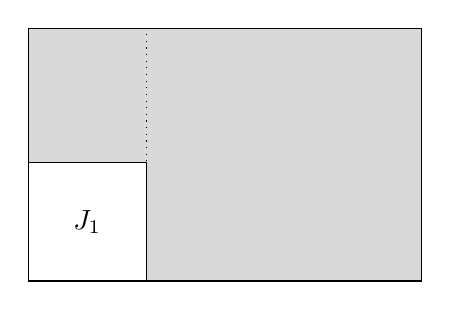
\begin{tikzpicture}
      \draw[fill=gray!30] (0,0) rectangle (5,3.21);
      \draw[fill=white] (0,0) rectangle (1.5,1.5) node[pos=.5] {$J_1$};
      \draw[dotted] (1.5,0) -- (1.5,3.21);
      %\draw[fill=gray!60] (5,0) rectangle (6,3.21);
    \end{tikzpicture}
    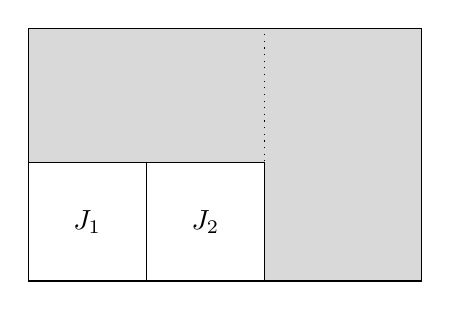
\begin{tikzpicture}
      \draw[fill=gray!30] (0,0) rectangle (5,3.21);
      \draw[fill=white] (0,0) rectangle (1.5,1.5) node[pos=.5] {$J_1$};
      \draw[fill=white] (1.5,0) rectangle (3,1.5) node[pos=.5] {$J_2$};
      \draw[dotted] (3,0) -- (3,3.21);
      %\draw[fill=gray!60] (5,0) rectangle (6,3.21);
    \end{tikzpicture}
    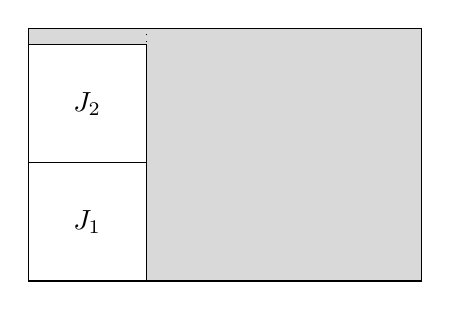
\begin{tikzpicture}
      \draw[fill=gray!30] (0,0) rectangle (5,3.21);
      \draw[fill=white] (0,0) rectangle (1.5,1.5) node[pos=.5] {$J_1$};
      \draw[fill=white] (0,1.5) rectangle (1.5,3) node[pos=.5] {$J_2$};
      \draw[dotted] (1.5,0) -- (1.5,3.21);
      %\draw[fill=gray!60] (5,0) rectangle (6,3.21);
    \end{tikzpicture}
    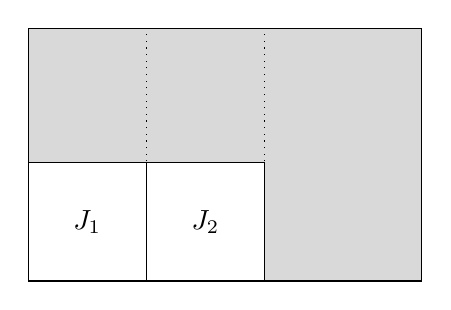
\begin{tikzpicture}
      \draw[fill=gray!30] (0,0) rectangle (5,3.21);
      \draw[fill=white] (0,0) rectangle (1.5,1.5) node[pos=.5] {$J_1$};
      \draw[fill=white] (1.5,0) rectangle (3,1.5) node[pos=.5] {$J_2$};
      \draw[dotted] (1.5,0) -- (1.5,3.21);
      \draw[dotted] (3,0) -- (3,3.21);
      %\draw[fill=gray!60] (5,0) rectangle (6,3.21);
    \end{tikzpicture}
  \end{center}
\end{frame}

\begin{frame}
  \frametitle{Transition}

  \begin{itemize}
    \item These search trees usually become very large when the depth increases \pause
    \item It is not possible to explore them exhaustively \pause
    \item We need to find smart ways to explore the most promising nodes
  \end{itemize}
\end{frame}

\section{Tree Search algorithms}

\begin{frame}
  \frametitle{Greedy algorithm}

  Select the best child until reaching a leaf.

  The value next to the nodes is the criteria used to compare them. The lesser the value, the better the node.

  \begin{center}
    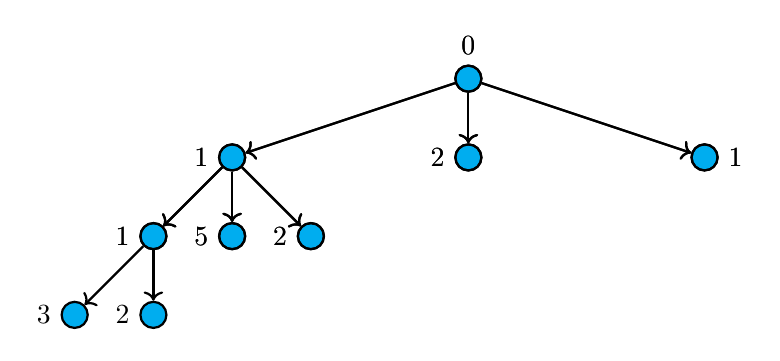
\begin{tikzpicture}
      \onslide<1>{%
        \node[draw=black, thick, circle, fill=cyan, label=above:0] (N1) at (0,0) {};
      }
      \onslide<2->{%
        \node[draw=black, thick, circle, label=above:0] (N1) at (0,0) {};
      }


      \onslide<2>{%
        \node[draw=black, thick, circle, fill=cyan, label=left:1] (N11) at (-3,-1) {};
        \draw [thick, draw=black, ->] (N1) -- (N11);
      }
      \onslide<3->{%
        \node[draw=black, thick, circle, label=left:1] (N11) at (-3,-1) {};
        \draw [thick, draw=black, ->] (N1) -- (N11);
      }

      \onslide<2>{%
        \node[draw=black, thick, circle, fill=cyan, label=left:2] (N12) at (0,-1) {};
        \draw [thick, draw=black, ->] (N1) -- (N12);
      }
      \onslide<3->{%
        \node[draw=black, thick, circle, label=left:2] (N12) at (0,-1) {};
        \draw [thick, draw=black, ->] (N1) -- (N12);
      }

      \onslide<2>{%
        \node[draw=black, thick, circle, fill=cyan, label=right:1] (N13) at (3,-1) {};
        \draw [thick, draw=black, ->] (N1) -- (N13);
      }
      \onslide<3->{%
        \node[draw=black, thick, circle, label=right:1] (N13) at (3,-1) {};
        \draw [thick, draw=black, ->] (N1) -- (N13);
      }


      \onslide<3>{%
        \node[draw=black, thick, circle, fill=cyan, label=left:1] (N111) at (-4,-2) {};
        \draw [thick, draw=black, ->] (N11) -- (N111);
      }
      \onslide<4->{%
        \node[draw=black, thick, circle, label=left:1] (N111) at (-4,-2) {};
        \draw [thick, draw=black, ->] (N11) -- (N111);
      }

      \onslide<3>{%
        \node[draw=black, thick, circle, fill=cyan, label=left:5] (N112) at (-3,-2) {};
        \draw [thick, draw=black, ->] (N11) -- (N112);
      }
      \onslide<4->{%
        \node[draw=black, thick, circle, label=left:5] (N112) at (-3,-2) {};
        \draw [thick, draw=black, ->] (N11) -- (N112);
      }

      \onslide<3>{%
        \node[draw=black, thick, circle, fill=cyan, label=left:2] (N113) at (-2,-2) {};
        \draw [thick, draw=black, ->] (N11) -- (N113);
      }
      \onslide<4->{%
        \node[draw=black, thick, circle, label=left:2] (N113) at (-2,-2) {};
        \draw [thick, draw=black, ->] (N11) -- (N113);
      }


      \onslide<4->{%
        \node[draw=black, thick, circle, fill=cyan, label=left:3] (N1111) at (-5,-3) {};
        \draw [thick, draw=black, ->] (N111) -- (N1111);
      }

      \onslide<4->{%
        \node[draw=black, thick, circle, fill=cyan, label=left:2] (N1112) at (-4,-3) {};
        \draw [thick, draw=black, ->] (N111) -- (N1112);
      }

    \end{tikzpicture}
  \end{center}

  \onslide<5->{%
    \begin{algorithmic}
      \Function{Greedy}{branching\_scheme}
      \State$\mathrm{node} \gets \mathrm{branching\_scheme.root}()$
      \While{$\mathrm{branching\_scheme.children}(\mathrm{node})$ is not empty}
      \State$\mathrm{node} \gets \text{\say{best} node from $\mathrm{branching\_scheme.children}(\mathrm{node})$}$
      \EndWhile{}
      \EndFunction{}
    \end{algorithmic}
  }
\end{frame}

\begin{frame}
  \frametitle{Greedy algorithm}

  Advantages:
  \begin{itemize}
    \item \pause Simple to understand and easy to implement
    \item \pause Fast
  \end{itemize}

  \pause Drawbacks:
  \begin{itemize}
    \item \pause Low quality solutions
  \end{itemize}
\end{frame}

\begin{frame}
  \frametitle{A / Best First Search algorithm}

  At each iteration, we expand the \say{best} node.

  \begin{center}
    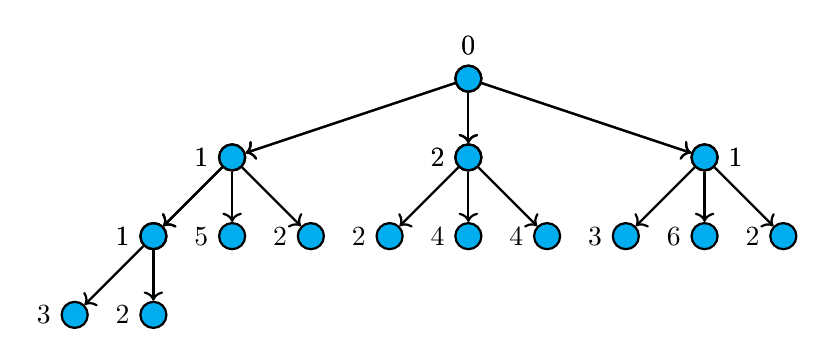
\begin{tikzpicture}
      \onslide<1>{%
        \node[draw=black, thick, circle, fill=cyan, label=above:0] (N1) at (0,0) {};
      }
      \onslide<2->{%
        \node[draw=black, thick, circle, label=above:0] (N1) at (0,0) {};
      }


      \onslide<2>{%
        \node[draw=black, thick, circle, fill=cyan, label=left:1] (N11) at (-3,-1) {};
        \draw [thick, draw=black, ->] (N1) -- (N11);
      }
      \onslide<3->{%
        \node[draw=black, thick, circle, label=left:1] (N11) at (-3,-1) {};
        \draw [thick, draw=black, ->] (N1) -- (N11);
      }

      \temporal<2-5>{}{%
        \node[draw=black, thick, circle, fill=cyan, label=left:2] (N12) at (0,-1) {};
        \draw [thick, draw=black, ->] (N1) -- (N12);
      }{%
        \node[draw=black, thick, circle, label=left:2] (N12) at (0,-1) {};
        \draw [thick, draw=black, ->] (N1) -- (N12);
      }

      \temporal<2-3>{}{%
        \node[draw=black, thick, circle, fill=cyan, label=right:1] (N13) at (3,-1) {};
        \draw [thick, draw=black, ->] (N1) -- (N13);
      }{%
        \node[draw=black, thick, circle, label=right:1] (N13) at (3,-1) {};
        \draw [thick, draw=black, ->] (N1) -- (N13);
      }


      \onslide<3-4>{%
        \node[draw=black, thick, circle, fill=cyan, label=left:1] (N111) at (-4,-2) {};
        \draw [thick, draw=black, ->] (N11) -- (N111);
      }
      \onslide<5->{%
        \node[draw=black, thick, circle, label=left:1] (N111) at (-4,-2) {};
        \draw [thick, draw=black, ->] (N11) -- (N111);
      }

      \onslide<3->{%
        \node[draw=black, thick, circle, fill=cyan, label=left:5] (N112) at (-3,-2) {};
        \draw [thick, draw=black, ->] (N11) -- (N112);
      }

      \onslide<3->{%
        \node[draw=black, thick, circle, fill=cyan, label=left:2] (N113) at (-2,-2) {};
        \draw [thick, draw=black, ->] (N11) -- (N113);
      }


      \onslide<4->{%
        \node[draw=black, thick, circle, fill=cyan, label=left:3] (N131) at (2,-2) {};
        \draw [thick, draw=black, ->] (N13) -- (N131);
      }

      \onslide<4->{%
        \node[draw=black, thick, circle, fill=cyan, label=left:6] (N132) at (3,-2) {};
        \draw [thick, draw=black, ->] (N13) -- (N132);
      }

      \onslide<4->{%
        \node[draw=black, thick, circle, fill=cyan, label=left:2] (N133) at (4,-2) {};
        \draw [thick, draw=black, ->] (N13) -- (N133);
      }


      \onslide<5->{%
        \node[draw=black, thick, circle, fill=cyan, label=left:3] (N1111) at (-5,-3) {};
        \draw [thick, draw=black, ->] (N111) -- (N1111);
      }

      \onslide<5->{%
        \node[draw=black, thick, circle, fill=cyan, label=left:2] (N1112) at (-4,-3) {};
        \draw [thick, draw=black, ->] (N111) -- (N1112);
      }


      \onslide<6->{%
        \node[draw=black, thick, circle, fill=cyan, label=left:2] (N121) at (-1,-2) {};
        \draw [thick, draw=black, ->] (N12) -- (N121);
      }

      \onslide<6->{%
        \node[draw=black, thick, circle, fill=cyan, label=left:4] (N122) at (-0,-2) {};
        \draw [thick, draw=black, ->] (N12) -- (N122);
      }

      \onslide<6->{%
        \node[draw=black, thick, circle, fill=cyan, label=left:4] (N123) at (1,-2) {};
        \draw [thick, draw=black, ->] (N12) -- (N123);
      }
    \end{tikzpicture}
  \end{center}

  \onslide<7->{%
    \begin{algorithmic}
      \Function{A}{branching\_scheme}
      \State $\mathrm{queue} \gets \{ \mathrm{branching\_scheme.root}() \}$
      \While {$\mathrm{queue}$ is not empty}
      \State $\mathrm{node} \gets \text{extract \say{best} node from $\mathrm{queue}$}$
      \State $\mathrm{queue} \gets \mathrm{queue} \cup \mathrm{branching\_scheme.children}(\mathrm{node})$
      \EndWhile
      \EndFunction
    \end{algorithmic}
  }
\end{frame}

\begin{frame}
  \frametitle{A / Best First Search algorithm}

  Advantages:
  \begin{itemize}
    \item \pause Simple to understand and easy to implement
    \item \pause If the guide is a bound, then it minimizes the number of nodes explored
  \end{itemize}

  \pause Drawbacks:
  \begin{itemize}
    \item \pause It might take a long time to reach leaves (full solutions)
    \item \pause The node queue quickly becomes too large
  \end{itemize}
\end{frame}

\begin{frame}
  \frametitle{Guides}

  For both Greedy and A algorithms, a criteria is required to compare nodes:
  \begin{itemize}
    \item Define and use the objective of the partial solutions:
      \begin{itemize}
        \item Examples:
          \begin{itemize}
            \item Travelling Salesman Problem: length of the partial tour
            \item 2D Knapsack: total profit of the currently selected items
          \end{itemize}
        \item Advantage: simple, might be good as a first approach
        \item Drawbacks: does not take into account the rest of the solution
          \begin{itemize}
            \item Travelling Salesman Problem: a forgotten location near the first ones
            \item 2D Knapsack: only big items remain
          \end{itemize}
      \end{itemize}
  \end{itemize}

  \pause
  \centering
  \begin{minipage}[t]{0.30\linewidth}
    \centering
    \def\svgwidth{\columnwidth}
    \input{travelling_salesman_solution_2.pdf_tex}
  \end{minipage}
  \begin{minipage}[t]{0.55\linewidth}
    \begin{center}
      \includegraphics[width=5.5cm]{knapsack_guide_4.png}
    \end{center}
  \end{minipage}
\end{frame}

\begin{frame}
  \frametitle{Guides}

  \begin{itemize}
    \item Criteria which takes into account what is and is not in the partial solution
  \end{itemize}

  \bigskip

  For the 2D guillotine Knapsack, first, instead of considering the profit $1 / \mathrm{profit}(S)$ of the partial solution $S$, we consider the $\mathrm{area}(S) / \mathrm{profit}(S)$ with $\mathrm{area}(S)$ defined as illustrated below:

  \begin{center}
    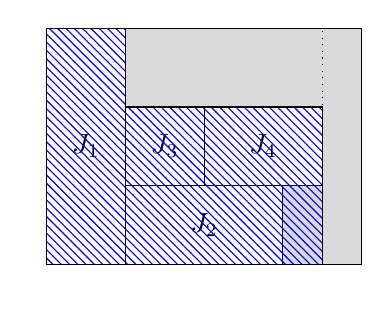
\begin{tikzpicture}
      \draw[fill=gray!30] (0,0) rectangle (4,3);
      \draw[fill=white] (0,0) rectangle (1,3) node[pos=.5] {$J_1$};
      \draw[fill=white] (1,0) rectangle (3,1) node[pos=.5] {$J_2$};
      \draw[fill=white] (1,1) rectangle (2,2) node[pos=.5] {$J_3$};
      \draw[fill=white] (2,1) rectangle (3.5,2) node[pos=.5] {$J_4$};
      \draw[dotted] (3.5,0) -- (3.5,3);
      \draw[dotted] (1,2) -- (3.5,2);
      \draw (3.5,0) node[anchor=north] {};
      \draw (1,0) node[anchor=north] {};
      \draw (2,0) node[anchor=north] {};
      \draw (0,1) node[anchor=east] {};
      \draw (0,2) node[anchor=east] {};
      \draw[pattern=north west lines, pattern color=blue] (0,0) rectangle (1,3);
      \draw[pattern=north west lines, pattern color=blue] (1,0) rectangle (3.5,2);
    \end{tikzpicture}
  \end{center}

  With this criteria, comparing nodes at different level of the tree makes more sense.
\end{frame}

\begin{frame}
  \frametitle{Guides}

  Then, to decrease the risk of packing all small items first, it is possible to introduce a bias in the guide:

  \begin{center}
    \begin{minipage}[t]{0.45\linewidth}
      \begin{center}
        \begin{displaymath}
          \frac{\mathrm{area}(S)}{\mathrm{profit(S)}}
        \end{displaymath}
        \includegraphics[width=5.5cm]{knapsack_guide_4.png}
      \end{center}
    \end{minipage}
    \hspace{0.25cm}
    \begin{minipage}[t]{0.45\linewidth}
      \begin{center}
        \begin{displaymath}
          \frac{\mathrm{area}(S)}{\mathrm{profit(S)}} \frac{1}{\mathrm{mean\_item\_area}(S)}
        \end{displaymath}
        \includegraphics[width=5.5cm]{knapsack_guide_5.png}
      \end{center}
    \end{minipage}
  \end{center}
  \bigskip

  Be careful about the computational complexity of the computation of the guide!
  In this example, it remains $O(1)$. More expensie guides may decrease the number of nodes explored.
\end{frame}

\begin{frame}
  \frametitle{Limited Discrepancy Search}

  Nodes are explored by increasing value of their discrepancy.

  \begin{center}
    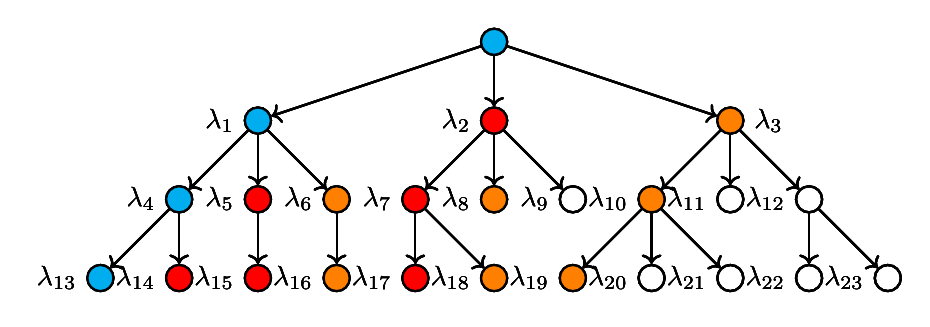
\begin{tikzpicture}
      \onslide<1>{%
        \node[draw=black, thick, circle] (N1) at (0,0) {};
        \node[draw=black, thick, circle, label=left:$\lambda_1$] (N11) at (-3,-1) {};
        \node[draw=black, thick, circle, label=left:$\lambda_2$] (N12) at (0,-1) {};
        \node[draw=black, thick, circle, label=right:$\lambda_3$] (N13) at (3,-1) {};
        \draw [thick, draw=black, ->] (N1) -- (N11);
        \draw [thick, draw=black, ->] (N1) -- (N12);
        \draw [thick, draw=black, ->] (N1) -- (N13);

        \node[draw=black, thick, circle, label=left:$\lambda_4$] (N111) at (-4,-2) {};
        \node[draw=black, thick, circle, label=left:$\lambda_5$] (N112) at (-3,-2) {};
        \node[draw=black, thick, circle, label=left:$\lambda_6$] (N113) at (-2,-2) {};
        \draw [thick, draw=black, ->] (N11) -- (N111);
        \draw [thick, draw=black, ->] (N11) -- (N112);
        \draw [thick, draw=black, ->] (N11) -- (N113);

        \node[draw=black, thick, circle, label=left:$\lambda_7$] (N121) at (-1,-2) {};
        \node[draw=black, thick, circle, label=left:$\lambda_8$] (N122) at (-0,-2) {};
        \node[draw=black, thick, circle, label=left:$\lambda_9$] (N123) at (1,-2) {};
        \draw [thick, draw=black, ->] (N12) -- (N121);
        \draw [thick, draw=black, ->] (N12) -- (N122);
        \draw [thick, draw=black, ->] (N12) -- (N123);

        \node[draw=black, thick, circle, label=left:$\lambda_{10}$] (N131) at (2,-2) {};
        \node[draw=black, thick, circle, label=left:$\lambda_{11}$] (N132) at (3,-2) {};
        \node[draw=black, thick, circle, label=left:$\lambda_{12}$] (N133) at (4,-2) {};
        \draw [thick, draw=black, ->] (N13) -- (N131);
        \draw [thick, draw=black, ->] (N13) -- (N132);
        \draw [thick, draw=black, ->] (N13) -- (N133);

        \node[draw=black, thick, circle, label=left:$\lambda_{13}$] (N1111) at (-5,-3) {};
        \node[draw=black, thick, circle, label=left:$\lambda_{14}$] (N1112) at (-4,-3) {};
        \draw [thick, draw=black, ->] (N111) -- (N1111);
        \draw [thick, draw=black, ->] (N111) -- (N1112);

        \node[draw=black, thick, circle, label=left:$\lambda_{15}$] (N1121) at (-3,-3) {};
        \draw [thick, draw=black, ->] (N112) -- (N1121);

        \node[draw=black, thick, circle, label=left:$\lambda_{16}$] (N1132) at (-2,-3) {};
        \draw [thick, draw=black, ->] (N113) -- (N1132);

        \node[draw=black, thick, circle, label=left:$\lambda_{17}$] (N1211) at (-1,-3) {};
        \node[draw=black, thick, circle, label=left:$\lambda_{18}$] (N1212) at (-0,-3) {};
        \draw [thick, draw=black, ->] (N121) -- (N1211);
        \draw [thick, draw=black, ->] (N121) -- (N1212);

        \node[draw=black, thick, circle, label=left:$\lambda_{19}$] (N1311) at (1,-3) {};
        \node[draw=black, thick, circle, label=left:$\lambda_{20}$] (N1312) at (2,-3) {};
        \node[draw=black, thick, circle, label=left:$\lambda_{21}$] (N1313) at (3,-3) {};
        \draw [thick, draw=black, ->] (N131) -- (N1311);
        \draw [thick, draw=black, ->] (N131) -- (N1312);
        \draw [thick, draw=black, ->] (N131) -- (N1313);

        \node[draw=black, thick, circle, label=left:$\lambda_{22}$] (N1331) at (4,-3) {};
        \node[draw=black, thick, circle, label=left:$\lambda_{23}$] (N1332) at (5,-3) {};
        \draw [thick, draw=black, ->] (N133) -- (N1331);
        \draw [thick, draw=black, ->] (N133) -- (N1332);
      }
      \onslide<2>{%
        \node[draw=black, thick, circle, fill=cyan] (N1) at (0,0) {};
        \node[draw=black, thick, circle, label=left:$\lambda_1$, fill=cyan] (N11) at (-3,-1) {};
        \node[draw=black, thick, circle, label=left:$\lambda_2$] (N12) at (0,-1) {};
        \node[draw=black, thick, circle, label=right:$\lambda_3$] (N13) at (3,-1) {};
        \draw [thick, draw=black, ->] (N1) -- (N11);
        \draw [thick, draw=black, ->] (N1) -- (N12);
        \draw [thick, draw=black, ->] (N1) -- (N13);

        \node[draw=black, thick, circle, label=left:$\lambda_4$, fill=cyan] (N111) at (-4,-2) {};
        \node[draw=black, thick, circle, label=left:$\lambda_5$] (N112) at (-3,-2) {};
        \node[draw=black, thick, circle, label=left:$\lambda_6$] (N113) at (-2,-2) {};
        \draw [thick, draw=black, ->] (N11) -- (N111);
        \draw [thick, draw=black, ->] (N11) -- (N112);
        \draw [thick, draw=black, ->] (N11) -- (N113);

        \node[draw=black, thick, circle, label=left:$\lambda_7$] (N121) at (-1,-2) {};
        \node[draw=black, thick, circle, label=left:$\lambda_8$] (N122) at (-0,-2) {};
        \node[draw=black, thick, circle, label=left:$\lambda_9$] (N123) at (1,-2) {};
        \draw [thick, draw=black, ->] (N12) -- (N121);
        \draw [thick, draw=black, ->] (N12) -- (N122);
        \draw [thick, draw=black, ->] (N12) -- (N123);

        \node[draw=black, thick, circle, label=left:$\lambda_{10}$] (N131) at (2,-2) {};
        \node[draw=black, thick, circle, label=left:$\lambda_{11}$] (N132) at (3,-2) {};
        \node[draw=black, thick, circle, label=left:$\lambda_{12}$] (N133) at (4,-2) {};
        \draw [thick, draw=black, ->] (N13) -- (N131);
        \draw [thick, draw=black, ->] (N13) -- (N132);
        \draw [thick, draw=black, ->] (N13) -- (N133);

        \node[draw=black, thick, circle, fill=cyan, label=left:$\lambda_{13}$] (N1111) at (-5,-3) {};
        \node[draw=black, thick, circle, label=left:$\lambda_{14}$] (N1112) at (-4,-3) {};
        \draw [thick, draw=black, ->] (N111) -- (N1111);
        \draw [thick, draw=black, ->] (N111) -- (N1112);

        \node[draw=black, thick, circle, label=left:$\lambda_{15}$] (N1121) at (-3,-3) {};
        \draw [thick, draw=black, ->] (N112) -- (N1121);

        \node[draw=black, thick, circle, label=left:$\lambda_{16}$] (N1132) at (-2,-3) {};
        \draw [thick, draw=black, ->] (N113) -- (N1132);

        \node[draw=black, thick, circle, label=left:$\lambda_{17}$] (N1211) at (-1,-3) {};
        \node[draw=black, thick, circle, label=left:$\lambda_{18}$] (N1212) at (-0,-3) {};
        \draw [thick, draw=black, ->] (N121) -- (N1211);
        \draw [thick, draw=black, ->] (N121) -- (N1212);

        \node[draw=black, thick, circle, label=left:$\lambda_{19}$] (N1311) at (1,-3) {};
        \node[draw=black, thick, circle, label=left:$\lambda_{20}$] (N1312) at (2,-3) {};
        \node[draw=black, thick, circle, label=left:$\lambda_{21}$] (N1313) at (3,-3) {};
        \draw [thick, draw=black, ->] (N131) -- (N1311);
        \draw [thick, draw=black, ->] (N131) -- (N1312);
        \draw [thick, draw=black, ->] (N131) -- (N1313);

        \node[draw=black, thick, circle, label=left:$\lambda_{22}$] (N1331) at (4,-3) {};
        \node[draw=black, thick, circle, label=left:$\lambda_{23}$] (N1332) at (5,-3) {};
        \draw [thick, draw=black, ->] (N133) -- (N1331);
        \draw [thick, draw=black, ->] (N133) -- (N1332);
      }
      \onslide<3>{%
        \node[draw=black, thick, circle, fill=cyan] (N1) at (0,0) {};
        \node[draw=black, thick, circle, label=left:$\lambda_1$, fill=cyan] (N11) at (-3,-1) {};
        \node[draw=black, thick, circle, label=left:$\lambda_2$, fill=red] (N12) at (0,-1) {};
        \node[draw=black, thick, circle, label=right:$\lambda_3$] (N13) at (3,-1) {};
        \draw [thick, draw=black, ->] (N1) -- (N11);
        \draw [thick, draw=black, ->] (N1) -- (N12);
        \draw [thick, draw=black, ->] (N1) -- (N13);

        \node[draw=black, thick, circle, label=left:$\lambda_4$, fill=cyan] (N111) at (-4,-2) {};
        \node[draw=black, thick, circle, label=left:$\lambda_5$, fill=red] (N112) at (-3,-2) {};
        \node[draw=black, thick, circle, label=left:$\lambda_6$] (N113) at (-2,-2) {};
        \draw [thick, draw=black, ->] (N11) -- (N111);
        \draw [thick, draw=black, ->] (N11) -- (N112);
        \draw [thick, draw=black, ->] (N11) -- (N113);

        \node[draw=black, thick, circle, label=left:$\lambda_7$, fill=red] (N121) at (-1,-2) {};
        \node[draw=black, thick, circle, label=left:$\lambda_8$] (N122) at (-0,-2) {};
        \node[draw=black, thick, circle, label=left:$\lambda_9$] (N123) at (1,-2) {};
        \draw [thick, draw=black, ->] (N12) -- (N121);
        \draw [thick, draw=black, ->] (N12) -- (N122);
        \draw [thick, draw=black, ->] (N12) -- (N123);

        \node[draw=black, thick, circle, label=left:$\lambda_{10}$] (N131) at (2,-2) {};
        \node[draw=black, thick, circle, label=left:$\lambda_{11}$] (N132) at (3,-2) {};
        \node[draw=black, thick, circle, label=left:$\lambda_{12}$] (N133) at (4,-2) {};
        \draw [thick, draw=black, ->] (N13) -- (N131);
        \draw [thick, draw=black, ->] (N13) -- (N132);
        \draw [thick, draw=black, ->] (N13) -- (N133);

        \node[draw=black, thick, circle, fill=cyan, label=left:$\lambda_{13}$] (N1111) at (-5,-3) {};
        \node[draw=black, thick, circle, fill=red, label=left:$\lambda_{14}$] (N1112) at (-4,-3) {};
        \draw [thick, draw=black, ->] (N111) -- (N1111);
        \draw [thick, draw=black, ->] (N111) -- (N1112);

        \node[draw=black, thick, circle, fill=red, label=left:$\lambda_{15}$] (N1121) at (-3,-3) {};
        \draw [thick, draw=black, ->] (N112) -- (N1121);

        \node[draw=black, thick, circle, label=left:$\lambda_{16}$] (N1132) at (-2,-3) {};
        \draw [thick, draw=black, ->] (N113) -- (N1132);

        \node[draw=black, thick, circle, fill=red, label=left:$\lambda_{17}$] (N1211) at (-1,-3) {};
        \node[draw=black, thick, circle, label=left:$\lambda_{18}$] (N1212) at (-0,-3) {};
        \draw [thick, draw=black, ->] (N121) -- (N1211);
        \draw [thick, draw=black, ->] (N121) -- (N1212);

        \node[draw=black, thick, circle, label=left:$\lambda_{19}$] (N1311) at (1,-3) {};
        \node[draw=black, thick, circle, label=left:$\lambda_{20}$] (N1312) at (2,-3) {};
        \node[draw=black, thick, circle, label=left:$\lambda_{21}$] (N1313) at (3,-3) {};
        \draw [thick, draw=black, ->] (N131) -- (N1311);
        \draw [thick, draw=black, ->] (N131) -- (N1312);
        \draw [thick, draw=black, ->] (N131) -- (N1313);

        \node[draw=black, thick, circle, label=left:$\lambda_{22}$] (N1331) at (4,-3) {};
        \node[draw=black, thick, circle, label=left:$\lambda_{23}$] (N1332) at (5,-3) {};
        \draw [thick, draw=black, ->] (N133) -- (N1331);
        \draw [thick, draw=black, ->] (N133) -- (N1332);
      }
      \onslide<4->{%
        \node[draw=black, thick, circle, fill=cyan] (N1) at (0,0) {};
        \node[draw=black, thick, circle, label=left:$\lambda_1$, fill=cyan] (N11) at (-3,-1) {};
        \node[draw=black, thick, circle, label=left:$\lambda_2$, fill=red] (N12) at (0,-1) {};
        \node[draw=black, thick, circle, label=right:$\lambda_3$, fill=orange] (N13) at (3,-1) {};
        \draw [thick, draw=black, ->] (N1) -- (N11);
        \draw [thick, draw=black, ->] (N1) -- (N12);
        \draw [thick, draw=black, ->] (N1) -- (N13);

        \node[draw=black, thick, circle, label=left:$\lambda_4$, fill=cyan] (N111) at (-4,-2) {};
        \node[draw=black, thick, circle, label=left:$\lambda_5$, fill=red] (N112) at (-3,-2) {};
        \node[draw=black, thick, circle, label=left:$\lambda_6$, fill=orange] (N113) at (-2,-2) {};
        \draw [thick, draw=black, ->] (N11) -- (N111);
        \draw [thick, draw=black, ->] (N11) -- (N112);
        \draw [thick, draw=black, ->] (N11) -- (N113);

        \node[draw=black, thick, circle, label=left:$\lambda_7$, fill=red] (N121) at (-1,-2) {};
        \node[draw=black, thick, circle, label=left:$\lambda_8$, fill=orange] (N122) at (-0,-2) {};
        \node[draw=black, thick, circle, label=left:$\lambda_9$] (N123) at (1,-2) {};
        \draw [thick, draw=black, ->] (N12) -- (N121);
        \draw [thick, draw=black, ->] (N12) -- (N122);
        \draw [thick, draw=black, ->] (N12) -- (N123);

        \node[draw=black, thick, circle, label=left:$\lambda_{10}$, fill=orange] (N131) at (2,-2) {};
        \node[draw=black, thick, circle, label=left:$\lambda_{11}$] (N132) at (3,-2) {};
        \node[draw=black, thick, circle, label=left:$\lambda_{12}$] (N133) at (4,-2) {};
        \draw [thick, draw=black, ->] (N13) -- (N131);
        \draw [thick, draw=black, ->] (N13) -- (N132);
        \draw [thick, draw=black, ->] (N13) -- (N133);

        \node[draw=black, thick, circle, fill=cyan, label=left:$\lambda_{13}$] (N1111) at (-5,-3) {};
        \node[draw=black, thick, circle, fill=red, label=left:$\lambda_{14}$] (N1112) at (-4,-3) {};
        \draw [thick, draw=black, ->] (N111) -- (N1111);
        \draw [thick, draw=black, ->] (N111) -- (N1112);

        \node[draw=black, thick, circle, fill=red, label=left:$\lambda_{15}$] (N1121) at (-3,-3) {};
        \draw [thick, draw=black, ->] (N112) -- (N1121);

        \node[draw=black, thick, circle, fill=orange, label=left:$\lambda_{16}$] (N1132) at (-2,-3) {};
        \draw [thick, draw=black, ->] (N113) -- (N1132);

        \node[draw=black, thick, circle, fill=red, label=left:$\lambda_{17}$] (N1211) at (-1,-3) {};
        \node[draw=black, thick, circle, fill=orange, label=left:$\lambda_{18}$] (N1212) at (-0,-3) {};
        \draw [thick, draw=black, ->] (N121) -- (N1211);
        \draw [thick, draw=black, ->] (N121) -- (N1212);

        \node[draw=black, thick, circle, fill=orange, label=left:$\lambda_{19}$] (N1311) at (1,-3) {};
        \node[draw=black, thick, circle, label=left:$\lambda_{20}$] (N1312) at (2,-3) {};
        \node[draw=black, thick, circle, label=left:$\lambda_{21}$] (N1313) at (3,-3) {};
        \draw [thick, draw=black, ->] (N131) -- (N1311);
        \draw [thick, draw=black, ->] (N131) -- (N1312);
        \draw [thick, draw=black, ->] (N131) -- (N1313);

        \node[draw=black, thick, circle, label=left:$\lambda_{22}$] (N1331) at (4,-3) {};
        \node[draw=black, thick, circle, label=left:$\lambda_{23}$] (N1332) at (5,-3) {};
        \draw [thick, draw=black, ->] (N133) -- (N1331);
        \draw [thick, draw=black, ->] (N133) -- (N1332);
      }
    \end{tikzpicture}
  \end{center}
\end{frame}

\begin{frame}
  \frametitle{Limited Discrepancy Search}

  Advantages:
  \begin{itemize}
    \item \pause Quickly reaches leaves
    \item \pause Works well with unbalanced trees
    \item \pause A node is only compared with its brothers:

      $\implies$ very easy to design a guide
  \end{itemize}

  \pause Drawbacks:
  \begin{itemize}
    \item \pause Does not work as well with more balanced trees

      A node is only compared with its brothers:

      $\implies$ succession of decisions are never challenged
  \end{itemize}
\end{frame}

\begin{frame}
  \frametitle{Beam Search}

  Breadth First Search with a maximum width (called \say{beam width}).

  At each stage, the \say{worst} nodes are discarded.

  \bigskip

  Example with a beam width of $5$

  \begin{center}
    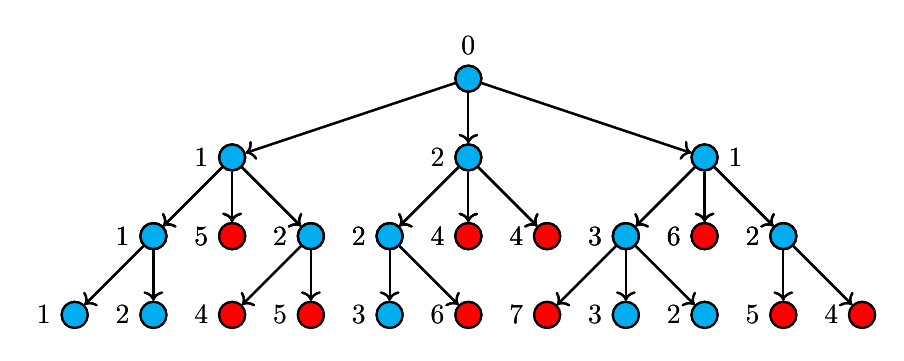
\begin{tikzpicture}
      \onslide<1>{\node[draw=black, thick, circle, fill=cyan, label=above:0] (N1) at (0,0) {};}
      \onslide<2->{\node[draw=black, thick, circle, label=above:0] (N1) at (0,0) {};}

      \onslide<2>{%
        \node[draw=black, thick, circle, fill=cyan, label=left:1] (N11) at (-3,-1) {};
        \node[draw=black, thick, circle, fill=cyan, label=left:2] (N12) at (0,-1) {};
        \node[draw=black, thick, circle, fill=cyan, label=right:1] (N13) at (3,-1) {};
        \draw [thick, draw=black, ->] (N1) -- (N11);
        \draw [thick, draw=black, ->] (N1) -- (N12);
        \draw [thick, draw=black, ->] (N1) -- (N13);
      }
      \onslide<3->{%
        \node[draw=black, thick, circle, label=left:1] (N11) at (-3,-1) {};
        \node[draw=black, thick, circle, label=left:2] (N12) at (0,-1) {};
        \node[draw=black, thick, circle, label=right:1] (N13) at (3,-1) {};
        \draw [thick, draw=black, ->] (N1) -- (N11);
        \draw [thick, draw=black, ->] (N1) -- (N12);
        \draw [thick, draw=black, ->] (N1) -- (N13);
      }

      \onslide<3>{%
        \node[draw=black, thick, circle, fill=cyan, label=left:1] (N111) at (-4,-2) {};
        \node[draw=black, thick, circle, fill=cyan, label=left:5] (N112) at (-3,-2) {};
        \node[draw=black, thick, circle, fill=cyan, label=left:2] (N113) at (-2,-2) {};
        \draw [thick, draw=black, ->] (N11) -- (N111);
        \draw [thick, draw=black, ->] (N11) -- (N112);
        \draw [thick, draw=black, ->] (N11) -- (N113);

        \node[draw=black, thick, circle, fill=cyan, label=left:2] (N121) at (-1,-2) {};
        \node[draw=black, thick, circle, fill=cyan, label=left:4] (N122) at (-0,-2) {};
        \node[draw=black, thick, circle, fill=cyan, label=left:4] (N123) at (1,-2) {};
        \draw [thick, draw=black, ->] (N12) -- (N121);
        \draw [thick, draw=black, ->] (N12) -- (N122);
        \draw [thick, draw=black, ->] (N12) -- (N123);

        \node[draw=black, thick, circle, fill=cyan, label=left:3] (N131) at (2,-2) {};
        \node[draw=black, thick, circle, fill=cyan, label=left:6] (N132) at (3,-2) {};
        \node[draw=black, thick, circle, fill=cyan, label=left:2] (N133) at (4,-2) {};
        \draw [thick, draw=black, ->] (N13) -- (N131);
        \draw [thick, draw=black, ->] (N13) -- (N132);
        \draw [thick, draw=black, ->] (N13) -- (N133);
      }
      \onslide<4>{%
        \node[draw=black, thick, circle, fill=cyan, label=left:1] (N111) at (-4,-2) {};
        \node[draw=black, thick, circle, fill=red, label=left:5] (N112) at (-3,-2) {};
        \node[draw=black, thick, circle, fill=cyan, label=left:2] (N113) at (-2,-2) {};
        \draw [thick, draw=black, ->] (N11) -- (N111);
        \draw [thick, draw=black, ->] (N11) -- (N112);
        \draw [thick, draw=black, ->] (N11) -- (N113);

        \node[draw=black, thick, circle, fill=cyan, label=left:2] (N121) at (-1,-2) {};
        \node[draw=black, thick, circle, fill=red, label=left:4] (N122) at (-0,-2) {};
        \node[draw=black, thick, circle, fill=red, label=left:4] (N123) at (1,-2) {};
        \draw [thick, draw=black, ->] (N12) -- (N121);
        \draw [thick, draw=black, ->] (N12) -- (N122);
        \draw [thick, draw=black, ->] (N12) -- (N123);

        \node[draw=black, thick, circle, fill=cyan, label=left:3] (N131) at (2,-2) {};
        \node[draw=black, thick, circle, fill=red, label=left:6] (N132) at (3,-2) {};
        \node[draw=black, thick, circle, fill=cyan, label=left:2] (N133) at (4,-2) {};
        \draw [thick, draw=black, ->] (N13) -- (N131);
        \draw [thick, draw=black, ->] (N13) -- (N132);
        \draw [thick, draw=black, ->] (N13) -- (N133);
      }
      \onslide<5->{%
        \node[draw=black, thick, circle, label=left:1] (N111) at (-4,-2) {};
        \node[draw=black, thick, circle, fill=red, label=left:5] (N112) at (-3,-2) {};
        \node[draw=black, thick, circle, label=left:2] (N113) at (-2,-2) {};
        \draw [thick, draw=black, ->] (N11) -- (N111);
        \draw [thick, draw=black, ->] (N11) -- (N112);
        \draw [thick, draw=black, ->] (N11) -- (N113);

        \node[draw=black, thick, circle, label=left:2] (N121) at (-1,-2) {};
        \node[draw=black, thick, circle, fill=red, label=left:4] (N122) at (-0,-2) {};
        \node[draw=black, thick, circle, fill=red, label=left:4] (N123) at (1,-2) {};
        \draw [thick, draw=black, ->] (N12) -- (N121);
        \draw [thick, draw=black, ->] (N12) -- (N122);
        \draw [thick, draw=black, ->] (N12) -- (N123);

        \node[draw=black, thick, circle, label=left:3] (N131) at (2,-2) {};
        \node[draw=black, thick, circle, fill=red, label=left:6] (N132) at (3,-2) {};
        \node[draw=black, thick, circle, label=left:2] (N133) at (4,-2) {};
        \draw [thick, draw=black, ->] (N13) -- (N131);
        \draw [thick, draw=black, ->] (N13) -- (N132);
        \draw [thick, draw=black, ->] (N13) -- (N133);
      }

      \onslide<5>{%
        \node[draw=black, thick, circle, fill=cyan, label=left:1] (N1111) at (-5,-3) {};
        \node[draw=black, thick, circle, fill=cyan, label=left:2] (N1112) at (-4,-3) {};
        \draw [thick, draw=black, ->] (N111) -- (N1111);
        \draw [thick, draw=black, ->] (N111) -- (N1112);

        \node[draw=black, thick, circle, fill=cyan, label=left:4] (N1131) at (-3,-3) {};
        \node[draw=black, thick, circle, fill=cyan, label=left:5] (N1132) at (-2,-3) {};
        \draw [thick, draw=black, ->] (N113) -- (N1131);
        \draw [thick, draw=black, ->] (N113) -- (N1132);

        \node[draw=black, thick, circle, fill=cyan, label=left:3] (N1211) at (-1,-3) {};
        \node[draw=black, thick, circle, fill=cyan, label=left:6] (N1212) at (-0,-3) {};
        \draw [thick, draw=black, ->] (N121) -- (N1211);
        \draw [thick, draw=black, ->] (N121) -- (N1212);

        \node[draw=black, thick, circle, fill=cyan, label=left:7] (N1311) at (1,-3) {};
        \node[draw=black, thick, circle, fill=cyan, label=left:3] (N1312) at (2,-3) {};
        \node[draw=black, thick, circle, fill=cyan, label=left:2] (N1313) at (3,-3) {};
        \draw [thick, draw=black, ->] (N131) -- (N1311);
        \draw [thick, draw=black, ->] (N131) -- (N1312);
        \draw [thick, draw=black, ->] (N131) -- (N1313);

        \node[draw=black, thick, circle, fill=cyan, label=left:5] (N1331) at (4,-3) {};
        \node[draw=black, thick, circle, fill=cyan, label=left:4] (N1332) at (5,-3) {};
        \draw [thick, draw=black, ->] (N133) -- (N1331);
        \draw [thick, draw=black, ->] (N133) -- (N1332);
      }
      \onslide<6->{%
        \node[draw=black, thick, circle, fill=cyan, label=left:1] (N1111) at (-5,-3) {};
        \node[draw=black, thick, circle, fill=cyan, label=left:2] (N1112) at (-4,-3) {};
        \draw [thick, draw=black, ->] (N111) -- (N1111);
        \draw [thick, draw=black, ->] (N111) -- (N1112);

        \node[draw=black, thick, circle, fill=red, label=left:4] (N1131) at (-3,-3) {};
        \node[draw=black, thick, circle, fill=red, label=left:5] (N1132) at (-2,-3) {};
        \draw [thick, draw=black, ->] (N113) -- (N1131);
        \draw [thick, draw=black, ->] (N113) -- (N1132);

        \node[draw=black, thick, circle, fill=cyan, label=left:3] (N1211) at (-1,-3) {};
        \node[draw=black, thick, circle, fill=red, label=left:6] (N1212) at (-0,-3) {};
        \draw [thick, draw=black, ->] (N121) -- (N1211);
        \draw [thick, draw=black, ->] (N121) -- (N1212);

        \node[draw=black, thick, circle, fill=red, label=left:7] (N1311) at (1,-3) {};
        \node[draw=black, thick, circle, fill=cyan, label=left:3] (N1312) at (2,-3) {};
        \node[draw=black, thick, circle, fill=cyan, label=left:2] (N1313) at (3,-3) {};
        \draw [thick, draw=black, ->] (N131) -- (N1311);
        \draw [thick, draw=black, ->] (N131) -- (N1312);
        \draw [thick, draw=black, ->] (N131) -- (N1313);

        \node[draw=black, thick, circle, fill=red, label=left:5] (N1331) at (4,-3) {};
        \node[draw=black, thick, circle, fill=red, label=left:4] (N1332) at (5,-3) {};
        \draw [thick, draw=black, ->] (N133) -- (N1331);
        \draw [thick, draw=black, ->] (N133) -- (N1332);
      }
    \end{tikzpicture}
  \end{center}
\end{frame}

\begin{frame}
  \frametitle{Beam Search}

  Advantages:
  \begin{itemize}
    \item \pause Good balance between the number of nodes explored at each depth
    \item \pause Only nodes at the same depth are compared with each other: easier to design a good guide
  \end{itemize}

  \pause Drawbacks:
  \begin{itemize}
    \item \pause How to choose the beam width?
  \end{itemize}
\end{frame}

\begin{frame}
  \frametitle{Dominances}

  Travelling Salesman Problem example:
  \begin{itemize}
    \item Node $N_1$: $1 \to 2 \to 3 \to 4$, length $10$
    \item Node $N_2$: $1 \to 3 \to 2 \to 4$, length $11$
  \end{itemize}

  We can safely prune Node $N_2$.

  \pause

  \bigskip

  More generally, let
  \begin{itemize}
    \item $\mathrm{visited}(N)$ be the list of visited locations of node $N$.
    \item $\mathrm{last}(N)$ be the last visited location of node $N$.
    \item $\mathrm{length}(N)$ be the length of the partial tour of node $N$.
  \end{itemize}

  Consider two nodes $N_1$ and $N_2$.
  If
  \begin{itemize}
    \item $\mathrm{visited}(N_1) \supseteq \mathrm{visited}(N_2)$
    \item $\mathrm{last}(N_1) = \mathrm{last}(N_2)$
    \item $\mathrm{length}(N_1) \le \mathrm{length}(N_2)$
  \end{itemize}
  then node $N_1$ dominates node $N_2$ and therefore node $N_2$ can be safely pruned.
\end{frame}

\begin{frame}
  \frametitle{A / Best First Search + Dynamic Programming}

  Each time a node is added to the queue:
  \begin{itemize}
    \item if it is dominated by another node which is in the queue, it is not added
    \item the nodes from the queue that it dominates are removed from the queue
  \end{itemize}

  \begin{center}
    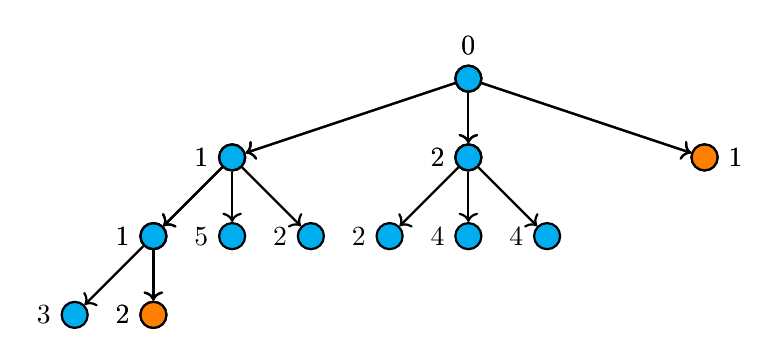
\begin{tikzpicture}
      \onslide<1>{%
        \node[draw=black, thick, circle, fill=cyan, label=above:0] (N1) at (0,0) {};
      }
      \onslide<2->{%
        \node[draw=black, thick, circle, label=above:0] (N1) at (0,0) {};
      }


      \onslide<2>{%
        \node[draw=black, thick, circle, fill=cyan, label=left:1] (N11) at (-3,-1) {};
        \draw [thick, draw=black, ->] (N1) -- (N11);
      }
      \onslide<3->{%
        \node[draw=black, thick, circle, label=left:1] (N11) at (-3,-1) {};
        \draw [thick, draw=black, ->] (N1) -- (N11);
      }

      \onslide<2-6>{%
        \node[draw=black, thick, circle, fill=cyan, label=left:2] (N12) at (0,-1) {};
        \draw [thick, draw=black, ->] (N1) -- (N12);
      }
      \onslide<7->{%
        \node[draw=black, thick, circle, label=left:2] (N12) at (0,-1) {};
        \draw [thick, draw=black, ->] (N1) -- (N12);
      }

      \onslide<2-3>{%
        \node[draw=black, thick, circle, fill=cyan, label=right:1] (N13) at (3,-1) {};
        \draw [thick, draw=black, ->] (N1) -- (N13);
      }
      \onslide<4->{%
        \node[draw=black, thick, circle, fill=orange, label=right:1] (N13) at (3,-1) {};
        \draw [thick, draw=black, ->] (N1) -- (N13);
      }


      \onslide<3-4>{%
        \node[draw=black, thick, circle, fill=cyan, label=left:1] (N111) at (-4,-2) {};
        \draw [thick, draw=black, ->] (N11) -- (N111);
      }
      \onslide<5->{%
        \node[draw=black, thick, circle, label=left:1] (N111) at (-4,-2) {};
        \draw [thick, draw=black, ->] (N11) -- (N111);
      }

      \onslide<3->{%
        \node[draw=black, thick, circle, fill=cyan, label=left:5] (N112) at (-3,-2) {};
        \draw [thick, draw=black, ->] (N11) -- (N112);
      }

      \onslide<3->{%
        \node[draw=black, thick, circle, fill=cyan, label=left:2] (N113) at (-2,-2) {};
        \draw [thick, draw=black, ->] (N11) -- (N113);
      }


      \onslide<5->{%
        \node[draw=black, thick, circle, fill=cyan, label=left:3] (N1111) at (-5,-3) {};
        \draw [thick, draw=black, ->] (N111) -- (N1111);
      }

      \onslide<5>{%
        \node[draw=black, thick, circle, fill=cyan, label=left:2] (N1112) at (-4,-3) {};
        \draw [thick, draw=black, ->] (N111) -- (N1112);
      } 
      \onslide<6->{%
        \node[draw=black, thick, circle, fill=orange, label=left:2] (N1112) at (-4,-3) {};
        \draw [thick, draw=black, ->] (N111) -- (N1112);
      } 


      \onslide<7->{%
        \node[draw=black, thick, circle, fill=cyan, label=left:2] (N121) at (-1,-2) {};
        \draw [thick, draw=black, ->] (N12) -- (N121);
      }

      \onslide<7->{%
        \node[draw=black, thick, circle, fill=cyan, label=left:4] (N122) at (-0,-2) {};
        \draw [thick, draw=black, ->] (N12) -- (N122);
      }

      \onslide<7->{%
        \node[draw=black, thick, circle, fill=cyan, label=left:4] (N123) at (1,-2) {};
        \draw [thick, draw=black, ->] (N12) -- (N123);
      }
    \end{tikzpicture}
  \end{center}
\end{frame}

\begin{frame}
  \frametitle{Beam Search + Dynamic Programming}

  Before discarding the \say{worst} nodes, the dominated ones are first removed.

  \bigskip

  Beam width: $5$

  \begin{center}
    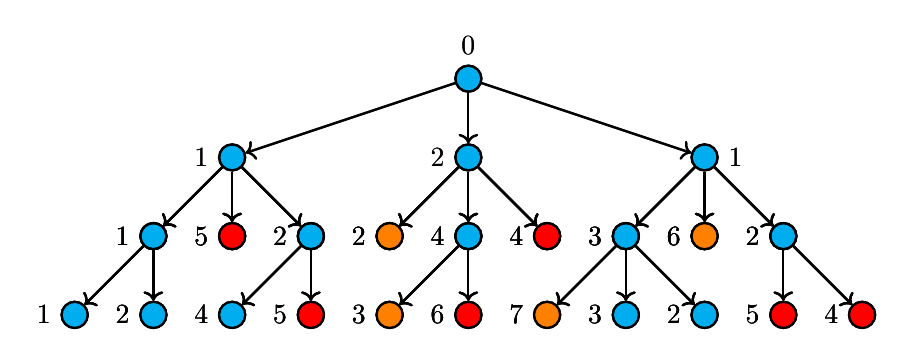
\begin{tikzpicture}
      \onslide<1>{\node[draw=black, thick, circle, fill=cyan, label=above:0] (N1) at (0,0) {};}
      \onslide<2->{\node[draw=black, thick, circle, label=above:0] (N1) at (0,0) {};}

      \onslide<2>{%
        \node[draw=black, thick, circle, fill=cyan, label=left:1] (N11) at (-3,-1) {};
        \node[draw=black, thick, circle, fill=cyan, label=left:2] (N12) at (0,-1) {};
        \node[draw=black, thick, circle, fill=cyan, label=right:1] (N13) at (3,-1) {};
        \draw [thick, draw=black, ->] (N1) -- (N11);
        \draw [thick, draw=black, ->] (N1) -- (N12);
        \draw [thick, draw=black, ->] (N1) -- (N13);
      }
      \onslide<3->{%
        \node[draw=black, thick, circle, label=left:1] (N11) at (-3,-1) {};
        \node[draw=black, thick, circle, label=left:2] (N12) at (0,-1) {};
        \node[draw=black, thick, circle, label=right:1] (N13) at (3,-1) {};
        \draw [thick, draw=black, ->] (N1) -- (N11);
        \draw [thick, draw=black, ->] (N1) -- (N12);
        \draw [thick, draw=black, ->] (N1) -- (N13);
      }

      \onslide<3>{%
        \node[draw=black, thick, circle, fill=cyan, label=left:1] (N111) at (-4,-2) {};
        \node[draw=black, thick, circle, fill=cyan, label=left:5] (N112) at (-3,-2) {};
        \node[draw=black, thick, circle, fill=cyan, label=left:2] (N113) at (-2,-2) {};
        \draw [thick, draw=black, ->] (N11) -- (N111);
        \draw [thick, draw=black, ->] (N11) -- (N112);
        \draw [thick, draw=black, ->] (N11) -- (N113);

        \node[draw=black, thick, circle, fill=cyan, label=left:2] (N121) at (-1,-2) {};
        \node[draw=black, thick, circle, fill=cyan, label=left:4] (N122) at (-0,-2) {};
        \node[draw=black, thick, circle, fill=cyan, label=left:4] (N123) at (1,-2) {};
        \draw [thick, draw=black, ->] (N12) -- (N121);
        \draw [thick, draw=black, ->] (N12) -- (N122);
        \draw [thick, draw=black, ->] (N12) -- (N123);

        \node[draw=black, thick, circle, fill=cyan, label=left:3] (N131) at (2,-2) {};
        \node[draw=black, thick, circle, fill=cyan, label=left:6] (N132) at (3,-2) {};
        \node[draw=black, thick, circle, fill=cyan, label=left:2] (N133) at (4,-2) {};
        \draw [thick, draw=black, ->] (N13) -- (N131);
        \draw [thick, draw=black, ->] (N13) -- (N132);
        \draw [thick, draw=black, ->] (N13) -- (N133);
      }
      \onslide<4>{%
        \node[draw=black, thick, circle, fill=cyan, label=left:1] (N111) at (-4,-2) {};
        \node[draw=black, thick, circle, fill=cyan, label=left:5] (N112) at (-3,-2) {};
        \node[draw=black, thick, circle, fill=cyan, label=left:2] (N113) at (-2,-2) {};
        \draw [thick, draw=black, ->] (N11) -- (N111);
        \draw [thick, draw=black, ->] (N11) -- (N112);
        \draw [thick, draw=black, ->] (N11) -- (N113);

        \node[draw=black, thick, circle, fill=orange, label=left:2] (N121) at (-1,-2) {};
        \node[draw=black, thick, circle, fill=cyan, label=left:4] (N122) at (-0,-2) {};
        \node[draw=black, thick, circle, fill=cyan, label=left:4] (N123) at (1,-2) {};
        \draw [thick, draw=black, ->] (N12) -- (N121);
        \draw [thick, draw=black, ->] (N12) -- (N122);
        \draw [thick, draw=black, ->] (N12) -- (N123);

        \node[draw=black, thick, circle, fill=cyan, label=left:3] (N131) at (2,-2) {};
        \node[draw=black, thick, circle, fill=orange, label=left:6] (N132) at (3,-2) {};
        \node[draw=black, thick, circle, fill=cyan, label=left:2] (N133) at (4,-2) {};
        \draw [thick, draw=black, ->] (N13) -- (N131);
        \draw [thick, draw=black, ->] (N13) -- (N132);
        \draw [thick, draw=black, ->] (N13) -- (N133);
      }
      \onslide<5>{%
        \node[draw=black, thick, circle, fill=cyan, label=left:1] (N111) at (-4,-2) {};
        \node[draw=black, thick, circle, fill=red, label=left:5] (N112) at (-3,-2) {};
        \node[draw=black, thick, circle, fill=cyan, label=left:2] (N113) at (-2,-2) {};
        \draw [thick, draw=black, ->] (N11) -- (N111);
        \draw [thick, draw=black, ->] (N11) -- (N112);
        \draw [thick, draw=black, ->] (N11) -- (N113);

        \node[draw=black, thick, circle, fill=orange, label=left:2] (N121) at (-1,-2) {};
        \node[draw=black, thick, circle, fill=cyan, label=left:4] (N122) at (-0,-2) {};
        \node[draw=black, thick, circle, fill=red, label=left:4] (N123) at (1,-2) {};
        \draw [thick, draw=black, ->] (N12) -- (N121);
        \draw [thick, draw=black, ->] (N12) -- (N122);
        \draw [thick, draw=black, ->] (N12) -- (N123);

        \node[draw=black, thick, circle, fill=cyan, label=left:3] (N131) at (2,-2) {};
        \node[draw=black, thick, circle, fill=orange, label=left:6] (N132) at (3,-2) {};
        \node[draw=black, thick, circle, fill=cyan, label=left:2] (N133) at (4,-2) {};
        \draw [thick, draw=black, ->] (N13) -- (N131);
        \draw [thick, draw=black, ->] (N13) -- (N132);
        \draw [thick, draw=black, ->] (N13) -- (N133);
      }
      \onslide<6->{%
        \node[draw=black, thick, circle, label=left:1] (N111) at (-4,-2) {};
        \node[draw=black, thick, circle, fill=red, label=left:5] (N112) at (-3,-2) {};
        \node[draw=black, thick, circle, label=left:2] (N113) at (-2,-2) {};
        \draw [thick, draw=black, ->] (N11) -- (N111);
        \draw [thick, draw=black, ->] (N11) -- (N112);
        \draw [thick, draw=black, ->] (N11) -- (N113);

        \node[draw=black, thick, circle, fill=orange, label=left:2] (N121) at (-1,-2) {};
        \node[draw=black, thick, circle, label=left:4] (N122) at (-0,-2) {};
        \node[draw=black, thick, circle, fill=red, label=left:4] (N123) at (1,-2) {};
        \draw [thick, draw=black, ->] (N12) -- (N121);
        \draw [thick, draw=black, ->] (N12) -- (N122);
        \draw [thick, draw=black, ->] (N12) -- (N123);

        \node[draw=black, thick, circle, label=left:3] (N131) at (2,-2) {};
        \node[draw=black, thick, circle, fill=orange, label=left:6] (N132) at (3,-2) {};
        \node[draw=black, thick, circle, label=left:2] (N133) at (4,-2) {};
        \draw [thick, draw=black, ->] (N13) -- (N131);
        \draw [thick, draw=black, ->] (N13) -- (N132);
        \draw [thick, draw=black, ->] (N13) -- (N133);
      }

      \onslide<6>{%
        \node[draw=black, thick, circle, fill=cyan, label=left:1] (N1111) at (-5,-3) {};
        \node[draw=black, thick, circle, fill=cyan, label=left:2] (N1112) at (-4,-3) {};
        \draw [thick, draw=black, ->] (N111) -- (N1111);
        \draw [thick, draw=black, ->] (N111) -- (N1112);

        \node[draw=black, thick, circle, fill=cyan, label=left:4] (N1131) at (-3,-3) {};
        \node[draw=black, thick, circle, fill=cyan, label=left:5] (N1132) at (-2,-3) {};
        \draw [thick, draw=black, ->] (N113) -- (N1131);
        \draw [thick, draw=black, ->] (N113) -- (N1132);

        \node[draw=black, thick, circle, fill=cyan, label=left:3] (N1221) at (-1,-3) {};
        \node[draw=black, thick, circle, fill=cyan, label=left:6] (N1222) at (-0,-3) {};
        \draw [thick, draw=black, ->] (N122) -- (N1221);
        \draw [thick, draw=black, ->] (N122) -- (N1222);

        \node[draw=black, thick, circle, fill=cyan, label=left:7] (N1311) at (1,-3) {};
        \node[draw=black, thick, circle, fill=cyan, label=left:3] (N1312) at (2,-3) {};
        \node[draw=black, thick, circle, fill=cyan, label=left:2] (N1313) at (3,-3) {};
        \draw [thick, draw=black, ->] (N131) -- (N1311);
        \draw [thick, draw=black, ->] (N131) -- (N1312);
        \draw [thick, draw=black, ->] (N131) -- (N1313);

        \node[draw=black, thick, circle, fill=cyan, label=left:5] (N1331) at (4,-3) {};
        \node[draw=black, thick, circle, fill=cyan, label=left:4] (N1332) at (5,-3) {};
        \draw [thick, draw=black, ->] (N133) -- (N1331);
        \draw [thick, draw=black, ->] (N133) -- (N1332);
      }
      \onslide<7>{%
        \node[draw=black, thick, circle, fill=cyan, label=left:1] (N1111) at (-5,-3) {};
        \node[draw=black, thick, circle, fill=cyan, label=left:2] (N1112) at (-4,-3) {};
        \draw [thick, draw=black, ->] (N111) -- (N1111);
        \draw [thick, draw=black, ->] (N111) -- (N1112);

        \node[draw=black, thick, circle, fill=cyan, label=left:4] (N1131) at (-3,-3) {};
        \node[draw=black, thick, circle, fill=cyan, label=left:5] (N1132) at (-2,-3) {};
        \draw [thick, draw=black, ->] (N113) -- (N1131);
        \draw [thick, draw=black, ->] (N113) -- (N1132);

        \node[draw=black, thick, circle, fill=orange, label=left:3] (N1221) at (-1,-3) {};
        \node[draw=black, thick, circle, fill=cyan, label=left:6] (N1222) at (-0,-3) {};
        \draw [thick, draw=black, ->] (N122) -- (N1221);
        \draw [thick, draw=black, ->] (N122) -- (N1222);

        \node[draw=black, thick, circle, fill=orange, label=left:7] (N1311) at (1,-3) {};
        \node[draw=black, thick, circle, fill=cyan, label=left:3] (N1312) at (2,-3) {};
        \node[draw=black, thick, circle, fill=cyan, label=left:2] (N1313) at (3,-3) {};
        \draw [thick, draw=black, ->] (N131) -- (N1311);
        \draw [thick, draw=black, ->] (N131) -- (N1312);
        \draw [thick, draw=black, ->] (N131) -- (N1313);

        \node[draw=black, thick, circle, fill=cyan, label=left:5] (N1331) at (4,-3) {};
        \node[draw=black, thick, circle, fill=cyan, label=left:4] (N1332) at (5,-3) {};
        \draw [thick, draw=black, ->] (N133) -- (N1331);
        \draw [thick, draw=black, ->] (N133) -- (N1332);
      }
      \onslide<8->{%
        \node[draw=black, thick, circle, fill=cyan, label=left:1] (N1111) at (-5,-3) {};
        \node[draw=black, thick, circle, fill=cyan, label=left:2] (N1112) at (-4,-3) {};
        \draw [thick, draw=black, ->] (N111) -- (N1111);
        \draw [thick, draw=black, ->] (N111) -- (N1112);

        \node[draw=black, thick, circle, fill=cyan, label=left:4] (N1131) at (-3,-3) {};
        \node[draw=black, thick, circle, fill=red, label=left:5] (N1132) at (-2,-3) {};
        \draw [thick, draw=black, ->] (N113) -- (N1131);
        \draw [thick, draw=black, ->] (N113) -- (N1132);

        \node[draw=black, thick, circle, fill=orange, label=left:3] (N1221) at (-1,-3) {};
        \node[draw=black, thick, circle, fill=red, label=left:6] (N1222) at (-0,-3) {};
        \draw [thick, draw=black, ->] (N122) -- (N1221);
        \draw [thick, draw=black, ->] (N122) -- (N1222);

        \node[draw=black, thick, circle, fill=orange, label=left:7] (N1311) at (1,-3) {};
        \node[draw=black, thick, circle, fill=cyan, label=left:3] (N1312) at (2,-3) {};
        \node[draw=black, thick, circle, fill=cyan, label=left:2] (N1313) at (3,-3) {};
        \draw [thick, draw=black, ->] (N131) -- (N1311);
        \draw [thick, draw=black, ->] (N131) -- (N1312);
        \draw [thick, draw=black, ->] (N131) -- (N1313);

        \node[draw=black, thick, circle, fill=red, label=left:5] (N1331) at (4,-3) {};
        \node[draw=black, thick, circle, fill=red, label=left:4] (N1332) at (5,-3) {};
        \draw [thick, draw=black, ->] (N133) -- (N1331);
        \draw [thick, draw=black, ->] (N133) -- (N1332);
      }
    \end{tikzpicture}
  \end{center}
\end{frame}

\begin{frame}
  \frametitle{Iterative Beam Search}

  How to choose the beam width:
  \begin{itemize}
    \item small: close to Greedy
    \item large: close to Breadth First Search
  \end{itemize}

  Iterative beam search:
  \begin{itemize}
    \item Succesive executions of a Beam Search while increasing the beam width: 1, 2, 4, 8, 16\dots
    \item Growth rate: between $1.25$ and $2$, small influence on the algorithm performances
    \item Anytime
  \end{itemize}
\end{frame}

\begin{frame}
  \frametitle{Heuristic Tree Search vs LP-based branch-and-bound}

  \begin{itemize}
    \pause
    \item An LP-based branch-and-bound is also a Tree Search:
      \begin{itemize}
        \item Root node: no variable bounds have been tightened
        \item Children: compute the relaxation, select a fractional variable, divide its domain in two and generate one child for each part
      \end{itemize}
    \pause
    \item The goal is to explore all nodes, or at least a good fraction of them
    \pause
    \item To reduce the number of nodes, an expensive bound is computed in each node
    \pause
    \item Works better than a Heuristic Tree Search approach if the bounds are strong
      \begin{itemize}
        \item Example: Arc-flow formulation of a Bin Packing Problem
      \end{itemize}
    \pause
    \item Performs poorly if the bounds are weak (a lot of time is spent in the nodes, but the number of nodes remains too high)
      \begin{itemize}
        \item Example: Two-dimensional bin packing
      \end{itemize}
  \end{itemize}
\end{frame}


\section{\texttt{treesearchsolverpy}}

\begin{frame}
  \frametitle{\texttt{treesearchsolverpy}}

  \begin{itemize}
    \item A package that simplifies the implementation of Tree Search based algorithms
    \item Written in \texttt{Python3} (original version in \texttt{C++})
    \item \url{https://github.com/fontanf/treesearchsolverpy}
    \item Install with: \texttt{pip3 install treesearchsolverpy}
    \item It includes an Iterative Beam Search + Dynamic Programming
    \item To solve a problem, one needs to create a \texttt{BranchingScheme} class that implements the requried methods (about 100--200 lines of code). Then:

      \texttt{iterative\_beam\_search(branching\_scheme)}
  \end{itemize}
\end{frame}

\begin{frame}
  \begin{itemize}
    \item For the branching scheme:
      \begin{itemize}
        \item \texttt{Node} class with \texttt{\_\_lt\_\_(self, other)} (guide)
        \item \texttt{root()} method
        \item \texttt{next\_child(father)} method
        \item \texttt{infertile(node)} method
        \item \texttt{leaf(node)} method
        \item \texttt{bound(node\_1, node\_2)} method
      \end{itemize}
    \item For the solution pool:
      \begin{itemize}
        \item \texttt{better(node\_1, node\_2)} method (main objective, not guide)
        \item \texttt{equals(node\_1, node\_2)} method (same solution, not same objective value)
      \end{itemize}
    \item For the dominances:
      \begin{itemize}
        \item \texttt{comparable(node)} method
        \item \texttt{Bucket} class with \texttt{\_\_init\_\_(self, node)}, \texttt{\_\_hash\_\_(self)} and \texttt{\_\_eq\_\_(self, other)}
        \item \texttt{dominates(node\_1, node\_2)} method (called only if both nodes are in the same bucket)
      \end{itemize}
    \item \texttt{display(node)} method
  \end{itemize}
\end{frame}

\section{Conclusion}

\begin{frame}
  \frametitle{Conclusion}

  \begin{itemize}
    \item Heuristic Tree Search: Branching Scheme + Tree Search algorithm (+ Guides, Dominances)
    \item New optimization method to add to your toolbox
    \item As for all other methods, does not work well for all problems
    \item Works well for medium-sized problems
      \begin{itemize}
        \item depth $\le 1000$
      \end{itemize}
    \item Works well for problems with many constraints
    \item Rather robust to the addition of new constraints
    \item Less robust to changes in the objective function
  \end{itemize}
\end{frame}

\maketitle

\end{document}

